\documentclass [listof=totoc,bibliography=totoc,german,a4paper,titlepage] {scrartcl}

\usepackage[english]{babel}
\usepackage{setspace}
\usepackage[paper=a4paper]{geometry}
\usepackage[utf8]{inputenc}
\usepackage{amsmath}
\usepackage{dsfont}
\usepackage{graphicx}
\usepackage{textcomp}
\usepackage{subfigure}
\usepackage{esvect}
\usepackage{pstricks}
\usepackage{floatflt}
\usepackage{SIunits}
\usepackage{amsopn}
\usepackage[percent]{overpic}

\setlength{\parskip}{6pt}
\setlength{\parindent}{0pt}

\onehalfspacing

\renewcommand{\thefigure}{\arabic{section}.\arabic{figure}}
\makeatletter \@addtoreset{figure}{section} \makeatother
\renewcommand{\thetable}{\arabic{section}.\arabic{table}}
\makeatletter \@addtoreset{table}{section} \makeatother
\renewcommand{\theequation}{\arabic{section}.\arabic{equation}}
\makeatletter \@addtoreset{equation}{section} \makeatother

\let\oldbibitem=\bibitem
\renewcommand{\bibitem}{%
\filbreak
\oldbibitem
}

\newenvironment{changemargin}[2]{%
  \begin{list}{}{%
    \setlength{\topsep}{0pt}%
    \setlength{\leftmargin}{#1}%
    \setlength{\rightmargin}{#2}%
    \setlength{\listparindent}{\parindent}%
    \setlength{\itemindent}{\parindent}%
    \setlength{\parsep}{\parskip}%
  }%
  \item[]}{\end{list}}


\newenvironment{mylisting}
{\begin{list}{}{\setlength{\leftmargin}{1em}}\item\scriptsize\bfseries}
{\end{list}}

\DeclareMathOperator{\grad}{grad}

\makeatletter
\let\divsymb\div              % make \IEEEendproof do same as \endproof
\let\div\@undefined                  % undefine \endproof
\makeatother

\DeclareMathOperator{\div}{div}

\begin{document}

%
%% Titelblatt
%%


\thispagestyle{empty} %% ohne Kopf- und Fusszeile, Seitennummer etc.

%% eigene Umgebung schaffen -> minipage
\begin{titlepage}     %% Anfang Sichtfenster

	\sffamily
	\begin{center}
		\vspace{1cm}
		
		\large{\textbf{Rheinisch-Westfälische Technische Hochschule Aachen\\Institut für Bildsame Formgebung}}
		
		\vspace{20mm}
				
		\Large{\textbf{Title bla blubb \\}}
		%\vspace{-0.35cm}
		\Large{\textbf{blubb bla}}
		
		\vspace{2cm}
		

		
		\LARGE{\textbf{Hauptseminar}} \\
		
		\vspace{1.5cm}
		
		\large{Paul Hibbe, B.Sc. \\ Matthias Nick, B.Sc.}\\
		
		\vspace{3cm}
		\end{center}
		
	%\large{Thema:\hspace{0.5cm}	Vergleich unterschiedlicher Dehnungsmessmethoden im quasistatischen Zugversuch\\ \hspace{2.0cm}}

	
\begin{center}
\large{Durchgeführt in der Abteilung Werkstoffmodellierung \\ im WS 2013/14}
\end{center}

\vspace{3cm}
\begin{tabbing}
\hspace*{3cm}\=\hspace{2cm}\=\kill
Betreuer: \>Univ. Prof. Dr.-Ing. Gerhard Hirt\\
          \>Dipl.-Ing. Thomas Henke\\
          \>Stephan Hojda, M.Sc.
\end{tabbing}
\end{titlepage} %% Ende Sichtfenster

\tableofcontents

\pagebreak

\section{Introduction}

Open-die forging is the oldest forging process and can be used to create a variety of final forms. It is an incremental, highly flexible metal forming process. The process typically involves two dies of simple geometry moving towards one another and thus forming the work piece. Open-die forging processes can be separated into four categories: upsetting, stretch forging, punching and hollow forging. This work, however, will focus on a stretch forging process.\cite{hbut}

Since the properties of the work piece depend strongly on the microstructure, methods to predict microstructural behaviour have been researched. The calculation of microstructure devolution based on the Finite Element modelling of the macroscopic mechanical process has proven to produce good results in this field. However, a systematic approach to test these results for open-die forging processes has yet to be undertaken. This work will focus on the microstructural modelling of a process that can easily be reproduced in reality.

Besides, the Finite Element results of the primarily used FEM package will be validated using other software. Software packages will be compared based on their usability and flexibility to describe open-die forging processes.


\section{Foundations}

\subsection{Open-die forging}
Open-die forging is the oldest forging process and can be used to create a variety of final forms. It is an incremental, highly flexible metal forming process primarily used today to prepare cast ingots for further closed-die forging or machining. The process typically involves two dies of simple geometry moving towards one another and thus forming the work piece. Open-die forging processes can be separated into four categories: upsetting, stretch forging, punching and hollow forging. \cite{hbut}


\section{Geometrische und thermische Grundlagen der Erwärmung mit Laser}

Zur Bestimmung der bei der Lasererwärmung eingetragenen Wärme ist die Betrachtung von zwei unterschiedlichen Teilaspekten notwendig: Zum Einen der Einfluss der Bewegungsgeschwindigkeit des Laserflecks, zum Anderen derjenige der Eigenschaften des verwendeten Werkstoffes.

\subsection{Geschwindigkeit des Laserbrennflecks}

Zur Bestimmung der Geschwindigkeit des Laserflecks wird das System in dreidimensionalen Koordinaten betrachtet. In diesen Koordinaten stellt sich die Bewegungsgeschwindigkeit $\vv{v_t}$ des Werkzeugs dar als:
\begin{equation}
 \vv{v_t} = \left(\begin{array}{c}v_{t,x}\\v_{t,y}\\0\end{array}\right)
 \label{eqn:toolvel3d}
\end{equation}

Weiterhin gilt für die Winkelgeschwindigkeit $\vv{\dot{\varphi}}$ der Bewegung des Laserflecks:
\begin{equation}
 \vv{\dot{\varphi}} = \left(\begin{array}{c}0\\0\\\dot{\varphi}\end{array}\right)
 \label{eqn:laserrotvel3d}
\end{equation}
 
Zudem ergibt sich aus der Geometrie des Aufbaus %(Abbildung \ref{img:geovel})
für den Radialvektor $\vv{r}$ mit der Entfernung $d_l$ des Laserflecks von der Rotationsachse:
\begin{equation}
\vv{r} = d_l\left(\begin{array}{c}-\sin\varphi\\\cos\varphi\\0\end{array}\right)
\label{eqn:radvec3d}
\end{equation}

% \begin{figure}[htbp]
%  \centering
%  \begin{pspicture}(8,5)
%   \psline{->}(4,1)(8,1)
%   \rput(8,0.6){x}
%   \psline{->}(4,1)(4,5)
%   \rput(3.6,5){y}
%   {
%    \SpecialCoor
%    \rput(4,1)
%    {
%     \psline(3.5;90)(0,0)(3.5;120)
%     \psarc{->}(0,0){3}{90}{120}
%     \rput[br](3.1;105){$\varphi$}
%    }
%   }
%  \end{pspicture}
%  \caption{Geometrie der Anordnung des Laserflecks}
%  \label{img:geovel}
% \end{figure}

Für den Geschwindigkeitsvektor $\vv{v_l}$ des Laserflecks gilt nun:
\begin{equation}
 \vv{v_l} = \vv{v_t} + \vv{\dot{\varphi}} \times \vv{r}
 \label{eqn:dotvelcomp}
\end{equation}

Einsetzen von Gleichungen \ref{eqn:toolvel3d}, \ref{eqn:laserrotvel3d} und \ref{eqn:radvec3d} in Gleichung \ref{eqn:dotvelcomp} und Umformen ergibt:
\begin{equation}
 \vv{v_l} = \left(\begin{array}{c}v_{t,x}\\v_{t,y}\\0\end{array}\right) - d_l\; \dot{\varphi} \left(\begin{array}{c}\cos\varphi\\\sin\varphi\\0\end{array}\right)
 \label{eqn:dotvelfin3d}
\end{equation}

Da das Problem im Prinzip zweidimensional ist und in Gleichung \ref{eqn:dotvelfin3d} die dritte Komponente immer null ist, liegt es nahe, die Gleichung in zwei Dimensionen darzustellen:
\begin{equation}
 \vv{v_l} = \left(\begin{array}{c}v_{t,x}\\v_{t,y}\end{array}\right) - d_l\; \dot{\varphi} \left(\begin{array}{c}\cos\varphi\\\sin\varphi\end{array}\right)
 \label{eqn:dotvelfin2d}
\end{equation}

Interessant ist jedoch nur der Betrag der Geschwindigkeit des Laserflecks, welcher sich wie folgt bestimmt:
\begin{equation}
 v_l = \left|\vv{v_l}\right| = \sqrt{\left(v_{t,x} - d_l\dot\varphi\cos\varphi\right)^2 + \left(v_{t,y} - d_l\dot\varphi\sin\varphi\right)^2}
 \label{eqn:dotvelabs}
\end{equation}

\label{sec:geotheory}

\subsection{Durch Laserstrahlung eingetragene Wärme}

Die Strahlungsenergie des Lasers wird im Blech in innere Energie in Form von Wärme umgewandelt. Laut \cite{atkins} gilt für die infinitesimale Temperaturänderung $dT$ durch die Änderung der inneren Energie $dU$ bei der spezifischen Wärmekapazität $C_{V,s}$ und konstantem Volumen:
\begin{equation}
  dT = \frac{dU}{mC_{V,s}}
  \label{eqn:specificheat}
\end{equation}

wobei $m$ die Masse des erwärmten Stoffes darstellt. Auf einem Teil eines Bleches der Dicke $d_s$, welches die Länge $l_e$ und die Breite $b_e$ besitzt (s. Abbildung \ref{img:element}), bestimmt sich die Masse über die Dichte $\rho$ zu:

\begin{equation}
 m = \rho V = \rho d_s l_e b_e
 \label{eqn:massgeometry}
\end{equation}

\begin{figure}[!btp]
 \centering
 \includegraphics[width=0.8\textwidth]{images/element}
 \caption{Skizze eines Volumenelements zur Bestimmung der Wärmekapazität}
 \label{img:element}
\end{figure}

Mit dieser Beziehung und Gleichung \ref{eqn:specificheat} ergibt sich für die Änderung der Temperatur:
\begin{equation}
  dT = \frac{dU}{\rho d_s l_e b_eC_{V,s}}
  \label{eqn:tempgeometry}
\end{equation}

Weiterhin ist die Leistung $P$ definiert als die Änderung der Energie mit der Zeit, also gilt:
\begin{equation}
  P = \frac{dU}{dt}\;\;\Leftrightarrow\;\; dU = Pdt
  \label{eqn:definitionpower}
\end{equation}

Laut \cite{laserheating} gilt für die absorbierte Leistung $P_a$:
\begin{equation}
  P_a = \alpha P_g
  \label{eqn:absorptivity}
\end{equation}

mit dem Absorptionsgrad $\alpha$ und der gesamten eingestrahlten Leistung $P_g$. Diese wiederum lässt sich mit $b_e'$, der Breite des vom Laserflecks getroffenen Teil des betrachteten Blechteils, sowie der Breite des gesamten Laserflecks $b_l$ und der Laserleistung $P_l$ abschätzen zu:
\begin{equation}
  P_g = \frac{b_e'}{b_l}P_l
  \label{eqn:powerfrac}
\end{equation}

Hierbei wird davon ausgegangen, dass die Laserleistung über die gesamte Breite des Laserflecks gleichverteilt ist. Einsetzen von Gleichung \ref{eqn:powerfrac} in Gleichung \ref{eqn:absorptivity} und dieser in \ref{eqn:definitionpower} ergibt:
\begin{equation}
  dU = \frac{b_e'}{b_l}\alpha P_l dt
  \label{eqn:energyofpower}
\end{equation} 

Dies wiederum ergibt mit Gleichung \ref{eqn:tempgeometry} einen Zusammenhang zwischen der Temperaturänderung und der Laserleistung:
\begin{equation}
  dT = \frac{1}{\rho d_s l_e b_eC_{V,s}} \frac{b_e'}{b_l}\alpha P_l dt = C \frac{b_e'}{b_l}\alpha P_l dt
  \label{eqn:dTofdt}
\end{equation}

Hierbei ist $C = \frac{1}{\rho d_s l_e b_eC_{V,s}}$ mit der Zeit konstant. Integrieren beider Seiten von $t'=0$ bis $t'=t$ ergibt:
\begin{equation}
  \Delta T = \int_{T(0)}^{T(t)} dT = \int_{0}^{t} C \frac{b_e'}{b_l}\alpha P_l dt' = C \frac{b_e'}{b_l} P_l \int_{0}^{t} \alpha dt'
  \label{eqn:integrationtemp}
\end{equation}

Dies ist zulässig, da laut \cite{laserheating} nur der Absorptionsgrad sich zwischen Raumtemperatur und Schmelztemperatur eines Metalls maßgeblich ändert. Dieser lässt sich mit der folgender Näherung beschreiben:

\begin{equation}
\alpha(T) = \alpha_0 + \alpha_1 T
\end{equation}

Dies würde jedoch eine Integration der rechten Seite von Gleichung \ref{eqn:integrationtemp} sehr kompliziert machen. Daher wird ein vereinfachter Absorptionsgrad $\alpha'$ eingeführt, der das Gesamtergebnis der Integration nicht beeinflusst, diese jedoch deutlich vereinfacht. Dazu lässt sich Gleichung \ref{eqn:dTofdt} umformen zu:

\begin{equation}
 \frac{\rho d_sl_eb_eC_{V,s}b_l}{b_e'}\frac{dT}{\alpha(T)} = c \frac{dT}{\alpha_0 + \alpha_1 T} = P_l dt
 \label{eqn:alphaintpreconst}
\end{equation}

wobei $c = \frac{\rho d_sl_eb_eC_{V,s}b_l}{b_e'P_l}$ als temperaturunabhängig gesehen werden kann. Integration ergibt:
\begin{equation}
  \int_{T_R}^{T_Z}c\frac{dT}{\alpha_0 + T \alpha_1} = c\frac{\ln\left(\alpha_0 T_Z + \alpha_1\right)-\ln\left(\alpha_0 T_R + \alpha_1\right)}{\alpha_1} = \Delta U = \int_0^t P_l dt'
\end{equation}

Wird nun $\alpha'$ eingeführt als 

\begin{equation}
\alpha' = \frac{\alpha_1 \Delta' T}{\ln\left(\alpha_0 T_Z + \alpha_1\right)-\ln\left(\alpha_0 T_R + \alpha_1\right)}
\label{eqn:alphas}
\end{equation}

mit $\Delta'T = T_Z-T_R$ der Differenz zwischen Zieltemperatur und Raumtemperatur, so ergibt sich, dass ein Ersetzen von $\alpha$ durch $\alpha'$ bei der Betrachtung der gesamten Temperaturdifferenz keinen Fehler einführt.

\begin{eqnarray}
  \int_{T_R}^{T_Z}c\frac{dT}{\alpha'} &=& c\int_{T_R}^{T_Z}\frac{\ln\left(\alpha_0 T_Z + \alpha_1\right)-\ln\left(\alpha_0 T_R + \alpha_1\right)}{\alpha_1 \Delta' T} dT\\\nonumber
   &= &c\frac{\ln\left(\alpha_0 T_Z + \alpha_1\right)-\ln\left(\alpha_0 T_R + \alpha_1\right)}{\alpha_1}\\
   &= &\int_{T_R}^{T_Z}c\frac{dT}{\alpha}
\end{eqnarray}

Somit kann durch diese vereinfachte Betrachtung die Entwicklung der Temperatur zwischen Raumtemperatur und Zieltemperatur nicht vorhergesagt werden. Dies führt in diesem Fall jedoch nicht zu Problemen, da einzig die zuzuführende Wärmemenge ausschlaggebend ist, die zur Zieltemperatur führt. Diese allerdings wird korrekt bestimmt. Für die Temperaturdifferenz ergibt sich:
\begin{equation}
  \Delta T = \frac{1}{\rho d_s l_e b_e C_{V,s}} \frac{b_e'}{b_l} P_l \alpha' \int_{0}^{t}  dt' = \frac{1}{\rho d_s l_e b_e C_{V,s}} \frac{b_e'}{b_l} P_l \alpha' t
  \label{eqn:integrated}
\end{equation}

Hier beschreibt $t$ die Zeit, in welcher der Laserstrahl das betrachtete Element über\-streicht. Diese lässt sich berechnen nach:
\begin{equation}
  t = \frac{l_e}{v_l}
  \label{eqn:elementtime}
\end{equation}

Somit wird Gleichung \ref{eqn:integrated} zu:
\begin{equation}
  \Delta T = \frac{\alpha'}{\rho d_s b_e C_{V,s}} \frac{b_e'}{b_l} \frac{P_l}{v_l}
  \label{eqn:prefinal}
\end{equation}

Da im Allgemeinen gilt $b_e << b_l$, ist davon auszugehen, dass der Effekt, der dadurch entsteht, dass jeweils zwei Elemente nur zum Teil vom Laserfleck überstrichen werden, gering ist, sich also $b_e' \approx b_e$ annehmen lässt. Somit ergibt sich aus Gl \ref{eqn:prefinal}
\begin{equation}
  \Delta T = \frac{\alpha'}{\rho d_s C_{V,s}b_l} \frac{P_l}{v_l} = c_P \frac{P_l}{v_l}\;\;\mbox{mit}\; c_P = \frac{\alpha'}{\rho d_s C_{V,s}b_l}
  \label{eqn:final} 
\end{equation}

wobei $c_P$ eine Konstante ist, die sich für den gesamten Prozess nicht ändert. Somit hängt die Temperaturdifferenz nur noch von der Laserleistung und der Geschwindigkeit des Laserbrennflecks ab.
\label{sec:heattheory}

\section{Model process}
This work deals with modeling of an open die forging process with multiple passes. The material used is a common stainless steel. The process parameters are orientated on a plan for forging a block with four passes given by the forging simulation software ForgeBase. Important process parameters, besides the flow curves, are for example the material data, the height reduction during every pass, the movement of the die, meaning the kinematics, the process temperature, etc. The detailed process conditions are discussed in the following chapters.\par

\subsection{Material data}
The material used is a 1.4301 (X5CrNiMo18-10) stainless steel. It is an austenitic steel which contains high quantities of the alloying elements chrome and nickel (Table 1). Therefore it is non-corrosive, acid- and heat-resistant. The field of application is widely spread and reaches from the automotive industry up to the chemical industry \cite{1.4301}.\par

The chemical composition (in weight-\%) of the material is as follows \cite{metallograf.de}:\begin{table}
 \centering
 \caption{Chemical composition of 1.4301}
 \begin{tabular}{|c|c|c|c|c|c|c|c|}
C[\%]&Cr[\%]&Ni[\%]&Si[\%]&Mn[\%]&P[\%]&S[\%]&N[\%]\\
 \hline
max 0,07&17,00-19,50&8,00-10,50&max 1,00&max. 2,00&max 0,045&max 0,03&max 0,11\\
 \end{tabular}
\end{table}\par

For the input in a simulation model the thermal material data is crucial, containing are the temperature depending thermal conductivity, the spec. heat capacity and the Young´s modul, see Figure \ref{img:thermalconductivity}, \ref{img:heatcapacity}, \ref{img:youngsmodul}.\par 

\begin{figure}[!htbp]
 \centering
 \includegraphics[width=0.8\textwidth]{images/thermalconductivity}
 \caption{Thermal conductivity of 1.4301}
 \label{img:thermalconductivity}
\end{figure}

\begin{figure}[!htbp]
 \centering
 \includegraphics[width=0.8\textwidth]{images/heatcapacity}
 \caption{Heat capacity of 1.4301}
 \label{img:heatcapacity}
\end{figure}

\begin{figure}[!htbp]
 \centering
 \includegraphics[width=0.8\textwidth]{images/youngsmodul}
 \caption{Young's modul of 1.4301}
 \label{img:youngsmodul}
\end{figure}

It is necessary that the data describes the whole temperature range of the process. Further parameters are set constant and are pictured in \ref{img:processparameter}\par 

\begin{table}
 \centering
 \caption{Constant process parameters (reference temperature 20°C)}
 \begin{tabular}{|c|c|c|}
 Poison&0,3&-\\
 \hline
 Thermal expansion&0,000012&[1/K]\\
 \hline
 Emissivity&0,7&-\\
 \hline
 Heat transfer coeff.&4,5&[W/(m²K)]\\
 \hline
 Friction coeff.&0,4&-\\
 \hline
 Dissipation&0,9&\%\\
 \hline
 \end{tabular}
\end{table}\par

\subsection{Forging plan (ForgeBase)}
The settings of the forging simulation are based on the calculation of the forging software ForgeBase. The simulations are done for a four passes process on a block (workpiece - WP) with the dimensions of 150mm in height as well as in width and 600mm in length. However, only 400mm of the length are forged. The rest is provided for the manipulator to hold and move the WP. The WP is set as a plastic solid and is meshed with a brick mesh with 12544 elements. The upper and lower dies are set as rigid object. The manipulator is set up as a spring with a stiffness of 175 N/mm and the maximum clamping force of 222,4 kN. For detailed dimensions of the upper and lower die, as of the manipulator see \\ref{Appendix1}.\par 

The passes in the simulation vary in height reduction and bite ratio. Between the passes the WP is rotated in positive and negative direction with 90° rotation angle. The bottom die is fixed, though the top die moves with a speed of 80mm/s.

\begin{figure}[!htbp]
 \centering
 \includegraphics[width=0.8\textwidth]{images/processsetup}
 \caption{Illustration of the process setup from DEFORM}
 \label{img:processsetup}
\end{figure}

\begin{table}
 \centering
 \caption{Forging plan from ForgeBase}
 \begin{tabular}{|c|c|c|c|c|c|c|c|}
 Pass Nr.&Reduction [mm]&Height 1[mm]&Width 1[mm]&Height 2[mm]&Width 2[mm]&Rotation [°]&Bite width [mm]\\
 \hline
 0&0&150&150&150&150&0&0\\
 \hline
 1&28&122&162&122&162&0&105\\
 \hline
 2&30&132&132&132&132&90&85\\
 \hline
 3&25&107&143&107&143&-90&92\\
 \hline
 4&27&116&116&116&116&90&75\\
 \hline
 \end{tabular}
\end{table}\par

Moreover, the heat treatment before and during the process is of great importance. Before the first pass starts, the WP gets heated up to 1200°C for 2 hours. It is vital, that the WP does have a homogeneous distribution. During the forging passes, heat is getting lost by the effects of emission and the heat transfers to the dies. Because of that, a second heat is necessary between the second and the third pass. The WP is heated up again to 1200°C within 1 hour. After the last pass the WP cools down upon air to room temperature.

\section{Previous work}

The described process has previously been investigated using Simufact.forming from simufact engineering gmbh. \textit{Zusammenfassung Ergebnisse Yuwei}

\section{Results of material modelling}

\section{Validation}

For the modelling of the described process, different software packages are available. Besides DEFORM3D, both FORGE from Transvalor, Mougins, France, and a combination of PEP (Pre- and Postprocessing Environment for Programmers) developed at IBF and LARSTRAN from LASSO Ingenieurgesellschaft mbH, Leinfelden, Germany have been used to validate the results. The packages differ in their ease of use and freedom in modelling. A comparison of both usability and results will be made here.

\subsection{FORGE}
FORGE, specifically FORGE3D, from Transvalor is a FEM software package catering primarily to industrial users. This can be seen in the easier to use and rather polished user interface. FORGE, like most packages, is split into a preprocessing tool, an equation system solver, and a postprocessing tool.

As a product for industrial customers, FORGE implements a fairly easy to use concept and various functions for simplifying the definition of die movement and kinematics. It provides predefined so-called Presses which, based on a few values such as initial height, final height, number of blows etc., create a basic kinematic for an open die forging process. While this provides an easy way to get results for simple processes, it makes the setup of specific, more advanced processes rather difficult.

While it is possible to define custom presses and use these to model die kinematics, this function is hardly documented in freely available documents such as FORGE's online help system. This, however, leads to defining kinematics via basic linear and rotational movement operations in cases that do not meet the predefined standard processes. Especially in academic surroundings, where processes vary widely, the combination of undocumented functions to define presses and limited freedom to access and modify the process in-process makes adequate process definition difficult.

Similar to the definition of kinematics and movements is the adaption of the available material data for FORGE. While an extensive material data base is available, import of new material data is not well documented. It is, however, possible to derive the data structure from exported files.

In FORGE, the process has been modelled symetrically with symmetry in the x-y and x-z planes. Apart from this, the model represents the real process in matters of die kinematics and work piece movement. That is, the die only moves in z direction while the work piece moves and rotates underneath it.

\subsubsection{Forging Forces}

The resulting forging forces acting on the dies are shown in diagrams \ref{img:forgforce_forge_p1} and \ref{img:forgforce_forge_p2} for passes 1 and 2 and passes 3 and 4 respectively. As is expected, the force required for forging rises with each blow. This can be explained by hardening mechanisms due to the introduced strain. The last blow of each pass requiring less force is due to the smaller bite length in the last blow. In general, forging forces between $1.5\mega\newton$ and $2.0\mega\newton$ seem realistic.

The diagram shows for pass 2 that a problem occurred in modelling. The peaks for the 2nd through 5th blow follow each other immediately, displaying a lack of waiting time in between. A closer examination of this will be seen below.

\begin{figure}[htbp]
  \centering
  \includegraphics[width=0.9\textwidth]{diagrams/force_pass1_forge}
  \caption{Forging forces for passes 1 and 2 as calculated by FORGE3D}
  \label{img:forgforce_forge_p1}
\end{figure}

\begin{figure}[htbp]
  \centering
  \includegraphics[width=0.9\textwidth]{diagrams/force_pass2_forge}
  \caption{Forging forces for passes 3 and 4 as calculated by FORGE3D}
  \label{img:forgforce_forge_p2}
\end{figure}

\subsubsection{Strain}

The effective strain in the core of the work piece after pass 4 is shown in diagram \ref{img:streff_forge}. A minimum value of 1.4 and a maximum value of 2.1 hint to a decent forging of the core.

\begin{figure}[htbp]
  \centering
  \includegraphics[width=0.9\textwidth]{diagrams/streff_forge}
  \caption{Effective strain in the core of the work piece after stroke 4 as calculated by FORGE3D}
  \label{img:streff_forge}
\end{figure}

\subsubsection{Temperature}

The temperature distribution in the core of the work piece after a cooling period of $120\minute$ is shown in diagram \ref{img:temp_forge}. Here, expectations are met as well by a low temperature at the head of the work piece, a fairly even distribution along its length and a rise in temperature at the end, which has not had any contact with the die.

\begin{figure}[htbp]
  \centering
  \includegraphics[width=0.9\textwidth]{diagrams/temperature_forge}
  \caption{Temperature distribution along the core after cooling as calculated by FORGE3D}
  \label{img:temp_forge}
\end{figure}

Diagram \ref{img:temp_time_forge} shows the temperature devolution of a node $100\milli\meter$ from the head of the work piece in its core. All stages of the process can clearly be seen here.

\begin{figure}[htbp]
  \centering
  \includegraphics[width=0.9\textwidth]{diagrams/temperature_time_forge}
  \caption{Temperature devolution of a point $100\milli\meter$ from the head in the core of the work piece as calculated by FORGE3D}
  \label{img:temp_time_forge}
\end{figure}


\subsection{PEP/LARSTRAN}

PEP/LARSTRAN is a combination of one pre- and postprocessing tool (PEP) and one solver (LARSTRAN). Both have been developed in an academic surrounding and accordingly provide more access to process variables during processing. On the other hand, a deeper understanding of FEM is necessary to use the system since values such as time step length and mesh element edge length are not calculated automatically but rather have to be input by the user.

Kinematics control is done via a so-called model program. Here, die movements, changes in die speed and other process variables are defined to happen at a given time step. While other systems provide the concept of manipulators which exert a certain restore force on the die to prevent unrealistic work piece movement due to singular die contact, PEP/LARSTRAN does not allow for such possibilities. Similar functionality has been achieved by defining a fixing of the work piece based on the number of contact nodes, but certain differences can still arise.

PEP/LARSTRAN die kinematics are based exclusively on the movement of the dies instead of the work piece. Since the concept of model programs does not allow for the definition of die movement according to the current work piece situation, however, it is not possible to even run one forging pass without stopping it and modifying the die movements. Moreover, the systems allows for only one ambient temperature, which means that each heating and cooling process and a combination of two forging passes have to be simulated separately and ambient temperature modified manually.

\subsubsection{Forging Forces}

\subsubsection{Strain}

\subsubsection{Temperature Distribution}

%\include{cadconcept}
\section{Summary}

It has been shown that the microstructural modelling of multi-pass open-die forging processes is possible. However, problems arise at small strain rates due to high resulting values for the dynamically recrystallized volume fraction. These, however, can be show to stem from a numerical effect at very small strain rates. This leads to SRX kinetics during the second heat that seem unrealistic. This leads to grain sizes that have to be evaluated critically.

The validation of the results from DEFORM has proven to be difficult. Differences in the approach of the various packages towards kinematics definition result in problems in recreating the process. However, where comparisons can be made, the systems still yield different results. This is especially obvious in the thermal modelling of the heating process, which is independent from die kinematics but still shows different results. Moreover, the resulting lengthening during the forging process differs between the used FEM packages, even leading to different numbers of blows needed to reach forging of the entire work piece.

In comparison, modelling in DEFORM using the cogging tool is a very handy way to setup an open-die forging model. Modelling open-die forging processes using FORGE is generally easy to do as well. However, more individual modelling leads to a sharp increase in the required effort. PEP/LARSTRAN, on the other hand, needs the user to have a deeper understanding of FEM as a concept and requires far more work in defining die kinematics.

\section{Outlook}

The results of microstucture modelling have shown that small strain rates result in large values for the dynamically recrystallized volume fraction. This effect is due to the limitations of using absolute thresholds for microstructural parameters. The models should be extended to give a more dynamic model which allows a bigger range of these paramenters.

Furthermore, a systematic approach to the comparison of various FEM packages with each other and with reality should involve, as a first step, the research of the capabilities of the involved packages and the development of an according model process. Also, an even more detailed process model should be set up, using the same time increments, mesh, boundary conditions etc.

Lastly, a validation of the results in a real process is necessary. This includes a validation of both the microstructural model with grain sizes measured during the process and the process parameters such as die forces and material temperature development.

%\appendix
%\include{usedsymbols}
\listoffigures
\newpage
\bibliographystyle{alphadin}
\bibliography{hauptseminar_hibbe_nick_2014}
\include{appendix}
\end{document}
